\documentclass[12pt]{article}


% Overall formatting
\sloppy
\let\cleardoublepage\clearpage % do not force chapters to start on odd pages


% Graphics
\usepackage{graphicx}
\DeclareGraphicsExtensions{.png,.pdf,.jpg}
\graphicspath{{Figures/}}


\usepackage[a4paper, total={16cm,25cm}]{geometry}



% Tables
\newlength{\mytabskip}   
\setlength{\mytabskip}{-1.5ex}
\newcommand{\tabrule}{\rule[\mytabskip]{0ex}{0ex}}
\usepackage{tabularx}
%\usepackage{longtable}


% bibliography stuff 
\usepackage{natbib}
\bibliographystyle{kluwer} 


\newcommand{\unit}[1]{\ensuremath{\mathrm{#1}}}
\newcommand{\degree}{\ensuremath{\mathrm{^\circ}}}

%\newcommand{\FIXME}[1]{{\sffamily \bfseries #1}}
\newcommand{\FIXME}[1]{{\sffamily {\bfseries \textcolor{red}{FIXME:} #1}}}


\hyphenation{EUMETSAT}
\hyphenation{Metop}



\begin{document}



\noindent
\textbf{\Large Arctic Weather Satellite: ???}  \vspace{8mm}\\
{\bf Patrick Eriksson, Simon Pfreundschuh and Inderpreet Kaur}\\
Department of Space, Earth and Environment\\
Chalmers University of Technology\\
SE-412\,96, Gothenburg, Sweden \vspace{10mm}

\section{Introduction}
%
\dots


\section{Data and methods}


\subsection{Fascod}
%
The Fascod dataset \citep{anderson1986afgl} is used to represent different
climate zones in overview calculations. The dataset consists of profiles of
pressure, temperature and volume mixing ratio profiles of various atmospheric
gases. Five climatoligies are used: tropical (TRO), mid-latitude summer (MLS),
mid-latitude winter (MLW), sub-arctic summer (SAS), and sub-arctic winter
(SAW). No hydrometeors are included in simulations involving Fascod.


\subsection{Bulk atmospheric profile database}
%
Refer to ICI and Robin's article.


\subsection{AWS}
%
Channels

The satellite is assumed to be at an altitude of 600\,km. 


\subsection{Radiative transfer simulations}
%
\subsubsection{ARTS}
%
All radiative transfer calculations are made by the Atmospheric Radiative
Transfer System (ARTS, \citet{eriksson:arts2:11,buehler:artst:18}), version
arts-2.3.????. Models and input used for absorption and hydrometeor properties
are described below. ARTS considers a spherical Earth by default. Scattering
calculations were made by ARTS's interface to the RT4 solver
\citep{evans1995microwavec}. Ocean/water and land emissivities ae taken from
TESSEM \citet{prigent2017sea} and TELSEM \citet{aires2011tool}, respectively.


\subsubsection{Absorption models}
%
The absorption of nitrogen is modelled following \citet{pwr:93}. Nitrogen has a
significant impact at least around 325\,GHz at dry conditions. Also oxygen
absorption follows \citet{pwr:93}. Oxygen is in this study mainly of concern
for the 89\,GHz CloudSat simulations. Liquid cloud water (LCW) is treated
purely absorbing, based on \citet{ellison2007permittivity}.

For water vapour the present settings in RTTOV are applied. That is, largely
MPM89 \citep{liebe:89} is followed, but some parameters for the 22 and 183\,GHz
transitions are replaced \citep{saunders2018update,turner2019amsutran}. A basic
comparison to RTTOV (12.?) was made (with MHS as assumed sensor) and an
agremment around or better than 0.?\,K was found.



\subsubsection{Hydrometeor properties}
%
\dots



\section{Results}

\subsection{Overview of the frequency bands}
%
The simulations involving Fascode were done using a fixed satellite observation
angle of 155$^\circ$ (from zenith) and a  


\begin{figure}[p]
  \centering
  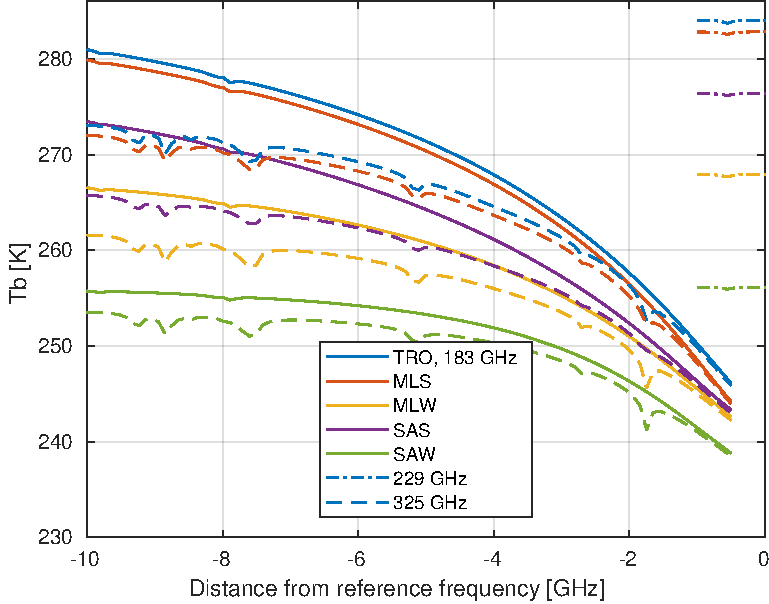
\includegraphics[width=0.7\textwidth]{fascod_tb_r000}
  \caption{dd}
  \label{fig:tb:r00}
\end{figure}
\begin{figure}[p]
  \centering
  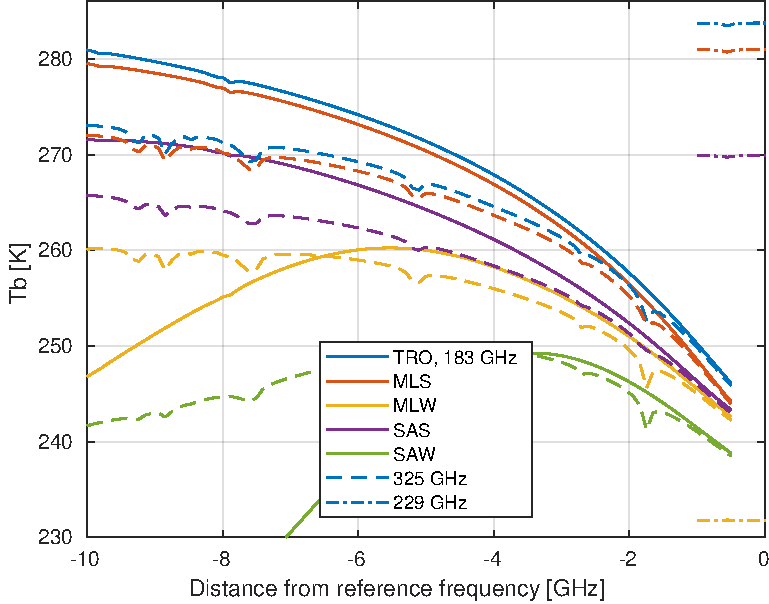
\includegraphics[width=0.7\textwidth]{fascod_tb_r050}
  \caption{Same as figure above, but with a surface reflectivity of 0.5.}
  \label{fig:tb:r00}
\end{figure}




\bibliography{j_abbr,references}

\end{document}
